\section{Rücktrieb und Stirnfläche}

In diesem Versuch soll der Rücktrieb in Abhängigkeit mit der Stirnfläche gemessen werden. Um so einen Teil der Formel für die Kraft in Formel \ref{Kraft} experimentell herzuleiten.

\subsection{Messaufbau}

Um diese Messung zu realisieren werden drei verschieden Große Kreisscheiben in den Luftstrom gebracht und die rücktreibenden Kräfte mit einem Kraftmesser gemessen.

\subsection{Auswertung}

Wir erhalten mit der Messung die Werte in Tabelle \ref{tab:Aufgabe2.1}. Die Werte für den Rücktrieb pro Fläche sind ähnlich, müssten aber unter idealen Bedingungen in der Theorie gleich sein. Allerdings lässt sich diese Abweichung einerseits auf die verschwindend kleine Messreihe zurückführen und auch auf die ungenaue Messmethode, da zum Beispiel Reibung eine große Rolle spielt. Was aber einen wesentlich größeren Effekt hat und auch die gemessene Werte erklären würde, ist die Tatsache, dass es deutlich mehr Verwirbelungen pro Fläche bei kleineren Scheiben im Vergleich zu größeren gibt, was wiederum zu einem größeren Wert für den Rücktrieb pro Fläche führt.

\begin{table}[h]
    \caption{Rücktreibende Kraft für verschieden große Kreisscheiben}
    \centering
    \begin{tabular}{c c c}
    \hline
    Radius Kreisscheibe     & Rücktrieb  & Rücktrieb / Fläche\\
    \hline
    \SI{4}{\centi\metre}     & \SI{0.53}{\newton} & \SI{105.44}{\newton\per\square\metre}\\[5pt]
    \SI{2.8}{\centi\metre}  &   \SI{0.31}{\newton} & \SI{125.86}{\newton\per\square\metre} \\[5pt]
    \SI{2}{\centi\metre}    &   \SI{0.17}{\newton} & \SI{135.28}{\newton\per\square\metre} \\[5pt]
    \hline
    \end{tabular}
    \label{tab:Aufgabe2.1}
\end{table}

\section{Rücktrieb und Strömungsgeschwindigkeit}

Mit diesem Versuch soll die Art der Abhängigkeit des Rücktriebs von der Strömungsgeschwindigkeit gezeigt werden. Dafür werden zwei der drei Kreisscheiben aus dem voherigen Versuch ausgewählt und der Rücktrieb für verschiedene Drehzahlen gemessen, die sich mit Hilfe Abb \ref{fig:Aeromechanik Versuch 1.2} in Windgeschwindigkeiten übersetzen lassen. Somit erhält man die gesuchte Abhängigkeit des Rücktriebs von der Windgeschwindigkeit.

\subsection{Messaufbau}

Die Kreisscheiben werden wie im voherigen Versuch mit einem Kraftmesser verbunden, um so die rücktreibende Kraft zu messen. Dann wird diese jeweils für Drehzahlen von 600 bis 2060 Umdrehungen pro Minute gemessen. Was Windgeschwindigkeiten von ungefähr \SI{6}{\metre\per\second} bis \SI{14.5}{\metre\per\second} entspricht.

\subsection{Auswertung}

Die durch die Messung erhaltenen Werte sind in den Grafiken  \ref{fig:Aeoreomechanik Versuch 2.21} und \ref{fig:Aeromechanik Versuch 2.22} grafisch dargestellt. Wie an den Kurven zu erkennen ist, folgt der Plot des Rücktriebs über der Geschwindigkeit einer Parabel und der Plot des Rücktriebs über dem dynamischen Druck einem linearen Zusammenhang. Daraus lässt sich folgern, dass der Rücktrieb mit dem Geschwindigkeitsquadrat und mit dem dynamischen Druck zu nimmt. Daraus kann man, zusammen mit dem vohergegangen Versuch das Gesetz für die Rücktreibende Kraft in Gleichung \ref{Kraft} folgern, dass in den folgenden Versuchen weiter Verwedung findet.

\begin{figure}[h]
    \centering
    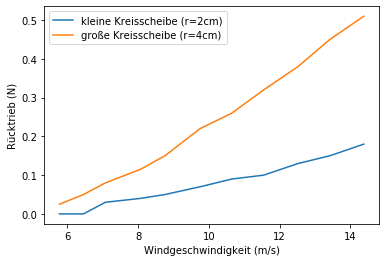
\includegraphics[scale=0.8]{Aeromechanik/Protokoll/fig/Aeromechanik Versuch 2.21.png}
    \caption{Rücktreibende Kraft für verschiedene Windgeschwindigkeiten für zwei Kreisscheiben mit unterschiedlichem Durchmesser}
    \label{fig:Aeoreomechanik Versuch 2.21}
\end{figure}

\begin{figure}[h]
    \centering
    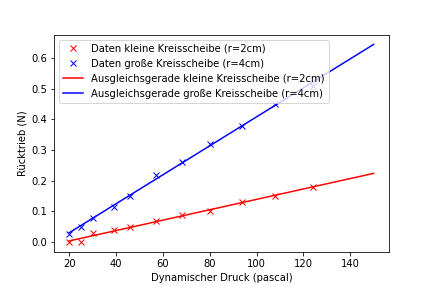
\includegraphics[scale= 0.8]{Aeromechanik/Protokoll/fig/Aeromechanik Versuch 2.22.png}
    \caption{Rücktreibende Kraft für verschiedene dynamische Drücke für zwei Kreisscheiben mit unterschiedlichem Durchmesser}
    \label{fig:Aeromechanik Versuch 2.22}
\end{figure}

\section{Rücktrieb und Körperform}

Wie in den vorhergegangen Versuchen ersichtlich ist der Rücktrieb proportional zur Fläche und zum dynamischen Druck. In diesem Versuch geht es nun darum zu demonstrieren, wie die Kraft auch von der Form des Körpers abhängig ist. 

\subsection{Messaufbau}

Dazu werden wie in den anderen Versuchen auch, die Körper in den Luftstrom geführt und deren rücktreibende Kraft mit einem Kraftmesser gemessen. Dies wird mit verschieden geformten Körpern bei einer konstanten Windgeschwindigkeit gemessen, um so auf die Abhängigkeit der Kraft von der Form des Körpers zu schließen. Verwendet werden in diesem Versuch: eine Halbkugel die in beiden Richtungen in den Luftstrom gehalten wird, eine Kugel und ein Stromlinienkörper in der vorgesehenen Richtung und um 180 Grad gedreht, jeweils mit gleicher Stirnfläche. Außerdem lässt sich mit den experimentell bestimmten Werte auch der Widerstandsbeiwert für die verschiedenen Körper berechnen.

\subsection{Auswertung}

Es ergeben sich die in der Tabelle aufgeführten Werte. Wie man an den Werten ablesen kann, stimmen die Werte für den Widerstandsbeiwert ziemlich gut mit den Literaturwerten überein, bis auf die beiden des Stromlinienkörpers, was aber vermutlich daran liegt, dass dieser einen sehr kleinen Rücktrieb hat und somit alle Fehler deutlicher zum Tragen kommmen. Ein Faktor dafür könnte beispielsweise sein, dass der Schlitten an dem der zu messende Körper befestigt ist nicht leichtgängig genug ist für kleine rücktreibenden Kräfte.

\begin{table}[]
    \caption{Rücktrieb für verschiedene Körper bei konstanter Windgeschwindigkeit von  \SI{14.38}{\metre\per\second} und daraus errechneter Widerstandsbeiwert}
    \centering
    \begin{tabular}{c c c c}
    \hline
    Körperform und Orientierung & Rücktrieb & Widerstandsbeiwert & Literaturwert\\
    \hline
    Halbkugel hohle Seite zum Gebläse   &   \SI{0.39}{\newton} & \SI{1.28}{\newton\per\pascal\square\metre} & \SI{1.33}{\newton\per\pascal\square\metre}  \\[5pt]
    Halbkugel hohle Seite vom Gebläse weg   &   \SI{0.12}{\newton} & \SI{0.39}{\newton\per\pascal\square\metre} &\SI{0.34}{\newton\per\pascal\square\metre}\\[5pt]
    Kugel & \SI{0.1}{\newton} & \SI{0.33}{\newton\per\pascal\square\metre} &\SI{0.45}{\newton\per\pascal\square\metre}\\[5pt]
    Stromlinienkörper richtig herum & \SI{0.04}{\newton} & \SI{0.13}{\newton\per\pascal\square\metre} & \SI{0.05}{\newton\per\pascal\square\metre}\\[5pt]
    Stromlinienkörper falsch herum & \SI{0.05}{\newton} & \SI{0.16}{\newton\per\pascal\square\metre} & \SI{0.04}{\newton\per\pascal\square\metre}\\[5pt]
    \hline
    \end{tabular}
    \label{tab:Versuch 2.3}
    Quelle Literaturwert: https://de.wikipedia.org/wiki/Strömungswiderstandskoeffizient
\end{table}

\section{Modellauto}

In diesem Versuch geht es darum, dass in den vorherigen Versuchen erlangte Wissen mit einer bekannten Anwendung der Aeromechanik zu verdeutlichen. Es geht darum den Widerstandsbeiwert oder den "C-W-Wert"  wie er umgangssprachlich auch genannt wird für zwei Modellautos zu berechnen. Dadurch, dass dieser nicht von der Größe der Stirnfläche abhängt, sondern noch von der Form des Körpers lässt sich somit auch ungefähr der echte Wert für diese Auto errechnen. 

\subsection{Messaufbau}

Um den Widerstandsbeiwert zu bestimmen, wird zuerst für die Plattform, auf die das Modellauto anschließend gestellt wird, der Rücktrieb gemessen. Dafür wird, wie in den vorangegangenen Versuchen auch, die Plattform am Schlitten befestigt und dieser wiederum mit dem Kraftmesser verbunden. Danach wird das Modellauto auf die Plattform gestellt und mit diesem erneut gemessen, jetzt kann man die Differenz der beiden Messungen benutzen um den Widerstandsbeiwert für das Modellauto zu berechnen und mit dem entsprechenden Literaturwert zu vergleichen.

\subsection{Auswertung}

Wie man an den experimentell ermittelten Werte im Vergleich zu den Literaturwerten sehen kann, haben diese eine relativ große Abweichung zueinander. Allerdings kann man dies dem ungenauen Messverfahren zuschreiben. Trotzdem kann man erkennen, dass man, mit einem geeigneteren Messverfahren, den Widerstandsbeiwert von Autos auch mit einem exakten Modell im Windkanal testen kann. Dieses Verfahren kommt auch in der Industrie zum Einsatz um Kosten zu senken, komplexe Strömungverhalten am Modell zu visualisieren und somit dieses zu verbessern, was wiederum die Effizienz von Autos steigert.

\begin{table}[]
    \caption{Widerstandsbeiwert von zwei Modellautos}
    \centering
    \begin{tabular}{c c c}
    \hline
    Modellauto  &   Widerstandsbeiwert (experimentell)  &   Widerstandsbeiwert (Literatur)  \\
    \hline
    Ford F-100     &    \SI{0.59}{\newton\per\pascal\square\metre}  & ca. \SI{0.5}{\newton\per\pascal\square\metre} \\[5pt]
    Chrysler PT-Cruiser & \SI{0.54}{\newton\per\pascal\square\metre}    &   \SI{0.37}{\newton\per\pascal\square\metre} \\[5pt]
    \hline
    \end{tabular}
    Quelle Widerstandsbeiwert (Literatur): http://rc.opelgt.org/indexcw.php
    \label{tab:my_label}
\end{table}